\documentclass[11pt,preprint]{elsarticle}

\usepackage{lmodern}
%%%% My spacing
\usepackage{setspace}
\setstretch{1.2}
\DeclareMathSizes{12}{14}{10}{10}

% Wrap around which gives all figures included the [H] command, or places it "here". This can be tedious to code in Rmarkdown.
\usepackage{float}
\let\origfigure\figure
\let\endorigfigure\endfigure
\renewenvironment{figure}[1][2] {
    \expandafter\origfigure\expandafter[H]
} {
    \endorigfigure
}

\let\origtable\table
\let\endorigtable\endtable
\renewenvironment{table}[1][2] {
    \expandafter\origtable\expandafter[H]
} {
    \endorigtable
}


\usepackage{ifxetex,ifluatex}
\usepackage{fixltx2e} % provides \textsubscript
\ifnum 0\ifxetex 1\fi\ifluatex 1\fi=0 % if pdftex
  \usepackage[T1]{fontenc}
  \usepackage[utf8]{inputenc}
\else % if luatex or xelatex
  \ifxetex
    \usepackage{mathspec}
    \usepackage{xltxtra,xunicode}
  \else
    \usepackage{fontspec}
  \fi
  \defaultfontfeatures{Mapping=tex-text,Scale=MatchLowercase}
  \newcommand{\euro}{€}
\fi

\usepackage{amssymb, amsmath, amsthm, amsfonts}

\def\bibsection{\section*{References}} %%% Make "References" appear before bibliography


\usepackage[numbers]{natbib}

\usepackage{longtable}
\usepackage[margin=2.3cm,bottom=2cm,top=2.5cm, includefoot]{geometry}
\usepackage{fancyhdr}
\usepackage[bottom, hang, flushmargin]{footmisc}
\usepackage{graphicx}
\numberwithin{equation}{section}
\numberwithin{figure}{section}
\numberwithin{table}{section}
\setlength{\parindent}{0cm}
\setlength{\parskip}{1.3ex plus 0.5ex minus 0.3ex}
\usepackage{textcomp}
\renewcommand{\headrulewidth}{0.2pt}
\renewcommand{\footrulewidth}{0.3pt}

\usepackage{array}
\newcolumntype{x}[1]{>{\centering\arraybackslash\hspace{0pt}}p{#1}}

%%%%  Remove the "preprint submitted to" part. Don't worry about this either, it just looks better without it:
\makeatletter
\def\ps@pprintTitle{%
  \let\@oddhead\@empty
  \let\@evenhead\@empty
  \let\@oddfoot\@empty
  \let\@evenfoot\@oddfoot
}
\makeatother

 \def\tightlist{} % This allows for subbullets!

\usepackage{hyperref}
\hypersetup{breaklinks=true,
            bookmarks=true,
            colorlinks=true,
            citecolor=blue,
            urlcolor=blue,
            linkcolor=blue,
            pdfborder={0 0 0}}


% The following packages allow huxtable to work:
\usepackage{siunitx}
\usepackage{multirow}
\usepackage{hhline}
\usepackage{calc}
\usepackage{tabularx}
\usepackage{booktabs}
\usepackage{caption}


\newenvironment{columns}[1][]{}{}

\newenvironment{column}[1]{\begin{minipage}{#1}\ignorespaces}{%
\end{minipage}
\ifhmode\unskip\fi
\aftergroup\useignorespacesandallpars}

\def\useignorespacesandallpars#1\ignorespaces\fi{%
#1\fi\ignorespacesandallpars}

\makeatletter
\def\ignorespacesandallpars{%
  \@ifnextchar\par
    {\expandafter\ignorespacesandallpars\@gobble}%
    {}%
}
\makeatother


% definitions for citeproc citations
\NewDocumentCommand\citeproctext{}{}
\NewDocumentCommand\citeproc{mm}{%
\href{\#cite.\detokenize{#1}}{#2}\nocite{#1}}

\makeatletter
% allow citations to break across lines
\let\@cite@ofmt\@firstofone
% avoid brackets around text for \cite:
\def\@biblabel#1{}
\def\@cite#1#2{{#1\if@tempswa , #2\fi}}
\makeatother
\newlength{\cslhangindent}
\setlength{\cslhangindent}{1.5em}
\newlength{\csllabelwidth}
\setlength{\csllabelwidth}{3em}
\newenvironment{CSLReferences}[2] % #1 hanging-indent, #2 entry-spacing
{\begin{list}{}{%
	\setlength{\itemindent}{0pt}
	\setlength{\leftmargin}{0pt}
	\setlength{\parsep}{0pt}
	% turn on hanging indent if param 1 is 1
	\ifodd #1
	\setlength{\leftmargin}{\cslhangindent}
	\setlength{\itemindent}{-1\cslhangindent}
	\fi
	% set entry spacing
	\setlength{\itemsep}{#2\baselineskip}}}
{\end{list}}

\usepackage{calc}
\newcommand{\CSLBlock}[1]{\hfill\break\parbox[t]{\linewidth}{\strut\ignorespaces#1\strut}}
\newcommand{\CSLLeftMargin}[1]{\parbox[t]{\csllabelwidth}{\strut#1\strut}}
\newcommand{\CSLRightInline}[1]{\parbox[t]{\linewidth - \csllabelwidth}{\strut#1\strut}}
\newcommand{\CSLIndent}[1]{\hspace{\cslhangindent}#1}


\urlstyle{same}  % don't use monospace font for urls
\setlength{\parindent}{0pt}
\setlength{\parskip}{6pt plus 2pt minus 1pt}
\setlength{\emergencystretch}{3em}  % prevent overfull lines
\setcounter{secnumdepth}{5}

%%% Use protect on footnotes to avoid problems with footnotes in titles
\let\rmarkdownfootnote\footnote%
\def\footnote{\protect\rmarkdownfootnote}
\IfFileExists{upquote.sty}{\usepackage{upquote}}{}

%%% Include extra packages specified by user

%%% Hard setting column skips for reports - this ensures greater consistency and control over the length settings in the document.
%% page layout
%% paragraphs
\setlength{\baselineskip}{12pt plus 0pt minus 0pt}
\setlength{\parskip}{12pt plus 0pt minus 0pt}
\setlength{\parindent}{0pt plus 0pt minus 0pt}
%% floats
\setlength{\floatsep}{12pt plus 0 pt minus 0pt}
\setlength{\textfloatsep}{20pt plus 0pt minus 0pt}
\setlength{\intextsep}{14pt plus 0pt minus 0pt}
\setlength{\dbltextfloatsep}{20pt plus 0pt minus 0pt}
\setlength{\dblfloatsep}{14pt plus 0pt minus 0pt}
%% maths
\setlength{\abovedisplayskip}{12pt plus 0pt minus 0pt}
\setlength{\belowdisplayskip}{12pt plus 0pt minus 0pt}
%% lists
\setlength{\topsep}{10pt plus 0pt minus 0pt}
\setlength{\partopsep}{3pt plus 0pt minus 0pt}
\setlength{\itemsep}{5pt plus 0pt minus 0pt}
\setlength{\labelsep}{8mm plus 0mm minus 0mm}
\setlength{\parsep}{\the\parskip}
\setlength{\listparindent}{\the\parindent}
%% verbatim
\setlength{\fboxsep}{5pt plus 0pt minus 0pt}



\begin{document}



\begin{frontmatter}  %

\title{QUESTION\_2}

% Set to FALSE if wanting to remove title (for submission)




\author[Add1]{Happy Matope}
\ead{25098209@sun.ac.za}





\address[Add1]{Stellenbosch University, South Africa}



\vspace{1cm}


\begin{keyword}
\footnotesize{
Size indexes \sep Active share \sep Realised volatility \sep GJR-GARCH
\sep Stratification \\
\vspace{0.3cm}
}
\footnotesize{
\textit{JEL classification} G11 \sep G12 \sep C58
}
\end{keyword}



\vspace{0.5cm}

\end{frontmatter}

\setcounter{footnote}{0}



%________________________
% Header and Footers
%%%%%%%%%%%%%%%%%%%%%%%%%%%%%%%%%
\pagestyle{fancy}
\chead{}
\rhead{Size Matters? Risk and Return Traits of South African Large, Mid
and Small Cap Indexes}
\lfoot{}
\rfoot{\footnotesize Page \thepage}
\lhead{}
%\rfoot{\footnotesize Page \thepage } % "e.g. Page 2"
\cfoot{}

%\setlength\headheight{30pt}
%%%%%%%%%%%%%%%%%%%%%%%%%%%%%%%%%
%________________________

\headsep 35pt % So that header does not go over title




\makeatletter
\@ifundefined{pandocbounded}{%
  \newsavebox\pandoc@box
  \newcommand*\pandocbounded[1]{%
    \sbox\pandoc@box{#1}%
    \Gscale@div\@tempa{\textheight}{\dimexpr\ht\pandoc@box+\dp\pandoc@box\relax}%
    \Gscale@div\@tempb{\linewidth}{\wd\pandoc@box}%
    \ifdim\@tempb\p@<\@tempa\p@\let\@tempa\@tempb\fi
    \ifdim\@tempa\p@<\p@\scalebox{\@tempa}{\usebox\pandoc@box}%
    \else\usebox{\pandoc@box}\fi}%
}{}
\makeatother

\begin{verbatim}
rm(list = ls()) # Clean your environment:
gc() # garbage collection - It can be useful to call gc after a large object has been removed, as this may prompt R to return memory to the operating system.
\end{verbatim}

\begin{verbatim}
##           used (Mb) gc trigger (Mb) max used (Mb)
## Ncells  567471 30.4    1270307 67.9   702077 37.5
## Vcells 1087032  8.3    8388608 64.0  1927755 14.8
\end{verbatim}

\begin{verbatim}
library(tidyverse)
\end{verbatim}

\begin{verbatim}
## Warning: package 'ggplot2' was built under R version 4.5.3
\end{verbatim}

\begin{verbatim}
## Warning: package 'purrr' was built under R version 4.5.3
\end{verbatim}

\begin{verbatim}
## Warning: package 'dplyr' was built under R version 4.5.3
\end{verbatim}

\begin{verbatim}
## -- Attaching core tidyverse packages ------------------------ tidyverse 2.0.0 --
## v dplyr     1.2.1     v readr     2.1.6
## v forcats   1.0.1     v stringr   1.6.0
## v ggplot2   4.0.3     v tibble    3.3.1
## v lubridate 1.9.5     v tidyr     1.3.2
## v purrr     1.2.2     
## -- Conflicts ------------------------------------------ tidyverse_conflicts() --
## x dplyr::filter() masks stats::filter()
## x dplyr::lag()    masks stats::lag()
## i Use the conflicted package (<http://conflicted.r-lib.org/>) to force all conflicts to become errors
\end{verbatim}

\begin{verbatim}
list.files('code/', full.names = T, recursive = T) %>% .[grepl('.R', .)] %>% as.list() %>% walk(~source(.))
\end{verbatim}

\section{\texorpdfstring{Introduction
\label{Introduction}}{Introduction }}\label{introduction}

Size indexes are often treated as interchangeable slices of the same
market. They are not. A large-cap index can carry a different sector
bet, a different degree of concentration and a different response to
market stress than a mid- or small-cap index. For a manager benchmarked
to the Capped SWIX (J433), these differences determine whether a size
tilt adds diversification or simply re-labels the same risk.

This report studies the JSE Large, Mid and Small cap indexes from
January 2015 to September 2026. It asks four questions:

\begin{enumerate}
\def\labelenumi{\arabic{enumi}.}
\tightlist
\item
  How do the indexes differ in sector exposure and stock concentration?
\item
  How far does each index sit from the Capped SWIX, measured by active
  share?
\item
  How do their returns and realised volatility compare, at index and
  constituent level?
\item
  Does the ranking of the size indexes change in stressed versus calm
  months?
\end{enumerate}

The analysis uses stratification, realised and GARCH volatility, rolling
returns and active share. Section \ref{Data} describes the data, Section
\ref{Method} the methods, Section \ref{Results} the results, and Section
\ref{Summary} summarises.

\section{\texorpdfstring{Data \label{Data}}{Data }}\label{data}

Table \ref{tab:data} lists the data. Monthly constituent weights for the
three size indexes and the Capped SWIX come from the index constituents
file. They are combined with daily returns for 277 JSE stocks to rebuild
each index, which lets us look inside the indexes rather than only at
their headline returns. The official index series (J200, J201, J202,
J433) are used only to check the rebuild. Four macro series are used for
stratification.

\begin{verbatim}
tab_print(Tab_Data, caption = "Data used", label = "tab:data", size = "\\scriptsize")
\end{verbatim}

\begin{table}[!htbp]
\centering
\caption{Data used} 
\label{tab:data}
\begingroup\scriptsize
\begin{tabular}{llllll}
  \hline
Series & Source & Frequency & Start & End & Detail \\ 
  \hline
Constituents \& weights: CappedSWIX & Monthly\_Index\_Constituents & Monthly & Dec 2014 & Aug 2026 & Avg. 144 stocks \\ 
  Constituents \& weights: LargeCaps & Monthly\_Index\_Constituents & Monthly & Dec 2014 & Aug 2026 & Avg. 40 stocks \\ 
  Constituents \& weights: MidCaps & Monthly\_Index\_Constituents & Monthly & Dec 2014 & Aug 2026 & Avg. 52 stocks \\ 
  Constituents \& weights: SmallCaps & Monthly\_Index\_Constituents & Monthly & Dec 2014 & Aug 2026 & Avg. 58 stocks \\ 
  Daily stock returns & Stock\_Returns\_Daily & Daily & Jan 2015 & Sep 2026 & 277 stocks \\ 
  Official index returns: J200 & Index\_Returns\_Daily & Daily & Jan 2015 & Sep 2026 & Validation \\ 
  Official index returns: J201 & Index\_Returns\_Daily & Daily & Jan 2015 & Sep 2026 & Validation \\ 
  Official index returns: J202 & Index\_Returns\_Daily & Daily & Jan 2015 & Sep 2026 & Validation \\ 
  Official index returns: J433 & Index\_Returns\_Daily & Daily & Jan 2015 & Sep 2026 & Validation \\ 
  Global policy uncertainty (EPU) & Macro series & Daily/monthly & Jan 2005 & Sep 2026 & Stratification \\ 
  Brent crude (realised vol) & Macro series & Daily/monthly & Jan 2005 & Sep 2026 & Stratification \\ 
  Rand implied vol (SAVIUSD) & Macro series & Daily/monthly & Sep 2013 & Sep 2026 & Stratification \\ 
  VIX (US implied vol) & Macro series & Daily/monthly & Jan 2005 & Sep 2026 & Stratification \\ 
   \hline
\end{tabular}
\endgroup
\end{table}

Three data treatments matter:

\begin{itemize}
\tightlist
\item
  \textbf{Missing sectors.} Sector labels are missing for many small-cap
  rows. Each stock is given the sector recorded for it elsewhere in the
  data; stocks with no record are labelled ``Unclassified''. This
  affects about 30\% of small-cap weight before 2020 and about 10\%
  afterwards.
\item
  \textbf{Weights.} Weights are rescaled to sum to one each month, after
  dropping the few holdings without return data.
\item
  \textbf{Returns.} For stock-level volatility, daily stock returns are
  capped at \(\pm 25\%\) to limit data errors.
\end{itemize}

Table \ref{tab:valid} shows that the rebuilt indexes track the official
series closely: daily correlations of 0.98 to 0.99, and annualised
returns within 0.3 percentage points.

\begin{verbatim}
tab_print(Validation %>% rename(Index = Tickers, `Ann. return (rebuilt)` = Ann_Ret_Rebuilt,
                                `Ann. return (official)` = Ann_Ret_Official,
                                `Tracking error` = Tracking_Error),
          caption = "Validation: rebuilt versus official index returns (daily)",
          label = "tab:valid")
\end{verbatim}

\begin{table}[!htbp]
\centering
\caption{Validation: rebuilt versus official index returns (daily)} 
\label{tab:valid}
\begingroup\footnotesize
\begin{tabular}{lrrrr}
  \hline
Index & Correlation & Ann. return (rebuilt) & Ann. return (official) & Tracking error \\ 
  \hline
CappedSWIX & 0.978 & 0.087 & 0.087 & 0.037 \\ 
  LargeCaps & 0.994 & 0.107 & 0.110 & 0.020 \\ 
  MidCaps & 0.994 & 0.074 & 0.073 & 0.018 \\ 
  SmallCaps & 0.982 & 0.106 & 0.103 & 0.027 \\ 
   \hline
\end{tabular}
\endgroup
\end{table}

Table \ref{tab:desc} reports descriptive statistics of the rebuilt daily
returns. All four series are negatively skewed and fat-tailed, and
normality is rejected for each (Jarque--Bera \(p<0.001\)). Small caps
stand out: the lowest daily volatility, but by far the fattest tails
(excess kurtosis of 23). That combination is the first hint that daily
small-cap volatility understates their true risk (Section \ref{Vol}).

\begin{verbatim}
tab_print(Tab_Desc,
          caption = "Descriptive statistics of daily index returns (Jan 2015 to Sep 2026)",
          label = "tab:desc")
\end{verbatim}

\begin{table}[!htbp]
\centering
\caption{Descriptive statistics of daily index returns (Jan 2015 to Sep 2026)} 
\label{tab:desc}
\begingroup\footnotesize
\begin{tabular}{lrrrrrrrr}
  \hline
Index & Obs & Mean (ann.) & SD (ann.) & Skewness & Excess kurtosis & Min & Max & Jarque-Bera p \\ 
  \hline
LargeCaps & 2935 & 0.101 & 0.187 & -0.459 & 5.455 & -0.094 & 0.074 & 0.000 \\ 
  MidCaps & 2935 & 0.071 & 0.172 & -0.935 & 9.479 & -0.099 & 0.061 & 0.000 \\ 
  SmallCaps & 2935 & 0.101 & 0.138 & -0.703 & 23.375 & -0.101 & 0.108 & 0.000 \\ 
  CappedSWIX & 2935 & 0.083 & 0.174 & -0.631 & 6.808 & -0.088 & 0.064 & 0.000 \\ 
   \hline
\end{tabular}
\endgroup
\end{table}

\section{\texorpdfstring{Methodology
\label{Method}}{Methodology }}\label{methodology}

\subsection{Index returns}\label{index-returns}

Each index return is built from its constituents. With \(w_{i,t-1}\) the
weight of stock \(i\) at the previous month-end, and weights drifting
with prices within the month:

\[
R_{p,t} = \sum_{i=1}^{N} w_{i,t-1} \, R_{i,t}, \qquad \sum_i w_{i,t-1} = 1.
\]

This is implemented with \texttt{rmsfuns::Safe\_Return.portfolio}, as in
the course practicals.

\subsection{Concentration and active
share}\label{concentration-and-active-share}

Concentration is measured by the top-10 weight and by the effective
number of stocks, the inverse of the Herfindahl--Hirschman index:

\[
N^{\text{eff}}_t = \frac{1}{\sum_i w_{i,t}^2}.
\]

\(N^{\text{eff}}\) is the number of equally weighted stocks that would
give the same concentration.

Active share measures how much of an index's holdings differ from the
benchmark (\citeproc{ref-cremers2009}{\textbf{cremers2009?}}):

\[
AS_t = \tfrac{1}{2}\sum_{i} \left| w^{\text{index}}_{i,t} - w^{\text{J433}}_{i,t} \right|.
\]

It runs from 0 (identical holdings) to 1 (no overlap).

\subsection{Rolling returns and realised
volatility}\label{rolling-returns-and-realised-volatility}

The rolling three-year annualised return is

\[
R^{(36)}_t = \Big(\prod_{s=t-35}^{t} (1+R_s)\Big)^{12/36} - 1.
\]

Realised volatility uses daily log returns \(r_t = \ln(1+R_t)\):

\[
\sigma^{RV}_t = \sqrt{252} \cdot \text{sd}\left(r_{t-251}, \dots, r_t\right).
\]

At constituent level, each stock's realised volatility is computed per
calendar year. The diversification ratio compares index volatility with
the average volatility of its stocks:

\[
DR = \frac{\sigma_{\text{index}}}{\sum_i \bar{w}_i \, \sigma_i}.
\]

A low \(DR\) means combining the stocks removes much of their individual
risk.

\subsection{GJR-GARCH model}\label{gjr-garch-model}

Volatility is also modelled with a GJR-GARCH(1,1)
(\citeproc{ref-glosten1993}{\textbf{glosten1993?}}), which lets bad news
raise volatility more than good news:

\[
r_t = \mu + \phi\, r_{t-1} + \varepsilon_t, \qquad \varepsilon_t = \sigma_t z_t, \qquad z_t \sim t_\nu,
\] \[
\sigma_t^2 = \omega + \left(\alpha + \gamma\, I_{t-1}\right)\varepsilon_{t-1}^2 + \beta\,\sigma_{t-1}^2, \qquad I_{t-1} = \begin{cases} 1 & \varepsilon_{t-1} < 0 \\ 0 & \text{otherwise.}\end{cases}
\]

\begin{itemize}
\tightlist
\item
  \(\gamma > 0\) is the leverage effect.
\item
  Persistence is \(\alpha + \beta + \gamma/2\), and the half-life of a
  volatility shock is \(\ln(0.5)/\ln(\text{persistence})\) days.
\item
  Student-\(t\) errors allow for the fat tails in Table \ref{tab:desc}.
\item
  Adequacy is checked with a Ljung--Box test on squared standardised
  residuals.
\end{itemize}

\subsection{Stale prices}\label{stale-prices}

Infrequent trading smooths measured returns
(\citeproc{ref-scholes1977}{\textbf{scholes1977?}};
\citeproc{ref-lo1990}{\textbf{lo1990?}}). Three indicators are used:

\begin{itemize}
\tightlist
\item
  the share of zero-return days;
\item
  the first-order autocorrelation of daily returns;
\item
  the ratio of volatility from monthly returns to volatility from daily
  returns
  (\(\text{sd}(R^{m})\sqrt{12} \,/\, \text{sd}(R^{d})\sqrt{252}\)). With
  serially independent returns this ratio is close to one; stale prices
  push it above one.
\end{itemize}

\subsection{Stratification}\label{stratification}

Following the course's stratification approach, months are sorted by a
stratifying series \(X_m\): J433 realised volatility, VIX, rand implied
volatility, oil realised volatility and global policy uncertainty. High
(low) months are the top (bottom) quintile of \(X_m\). Daily returns are
winsorised at the 1st and 99th percentiles. For each index:

\begin{itemize}
\tightlist
\item
  the volatility ratio is \(\sigma_{\text{High}}/\sigma_{\text{Full}}\);
\item
  the monthly excess return over J433 is compared between High and Low
  months with a Welch two-sample \(t\)-test.
\end{itemize}

\section{\texorpdfstring{Results
\label{Results}}{Results }}\label{results}

\subsection{Sector exposure}\label{sector-exposure}

The three indexes carry very different sector bets (Figure
\ref{Figure1}, Table \ref{tab:sector}).

\begin{itemize}
\tightlist
\item
  \textbf{Large caps carry the market's Resources risk.} Resources rose
  from about 20\% of the index in 2015--19 to 35--40\% by 2026, led by
  the gold miners; Gold Fields and AngloGold Ashanti are now the two
  largest holdings.
\item
  \textbf{Mid caps have shifted from Property towards Financials}, with
  Financials more than doubling, from 12\% to 28\%.
\item
  \textbf{Small caps are effectively a Property and Industrials index},
  with little exposure to Resources or Financials.
\end{itemize}

\begin{verbatim}
fmxdat::finplot(g_sector, x.date.dist = "2 years", x.date.type = "%Y",
                x.vert = TRUE, y.pct = TRUE, y.pct_acc = 1)
\end{verbatim}

\begin{figure}
\centering
\pandocbounded{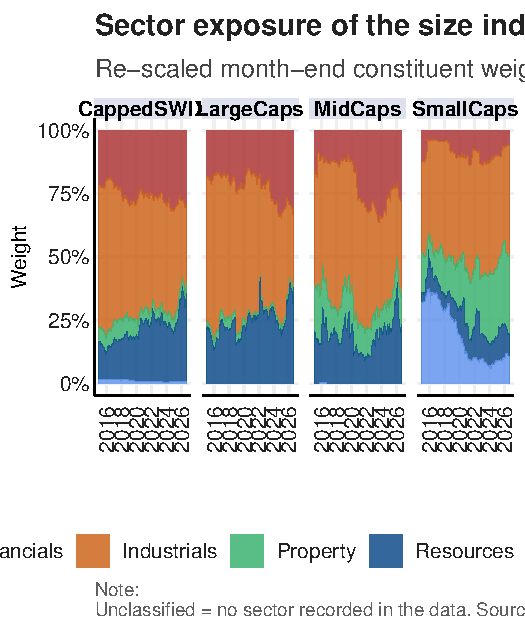
\includegraphics[keepaspectratio,alt={Sector exposure of the size indexes }]{Question2_files/figure-latex/Figure1-1.pdf}}
\caption{Sector exposure of the size indexes \label{Figure1}}
\end{figure}

\begin{verbatim}
tab_print(Sector_Table %>% rename(Index = Fund),
          caption = "Average sector weights by period", label = "tab:sector",
          size = "\\scriptsize")
\end{verbatim}

\begin{table}[!htbp]
\centering
\caption{Average sector weights by period} 
\label{tab:sector}
\begingroup\scriptsize
\begin{tabular}{llrrrrr}
  \hline
Index & Period & Financials & Industrials & Property & Resources & Unclassified \\ 
  \hline
CappedSWIX & 2015-2019 & 0.241 & 0.522 & 0.071 & 0.152 & 0.013 \\ 
  CappedSWIX & 2020-2026 & 0.273 & 0.429 & 0.045 & 0.247 & 0.006 \\ 
  LargeCaps & 2015-2019 & 0.196 & 0.569 & 0.033 & 0.202 & 0.000 \\ 
  LargeCaps & 2020-2026 & 0.244 & 0.463 & 0.018 & 0.276 & 0.000 \\ 
  MidCaps & 2015-2019 & 0.124 & 0.521 & 0.156 & 0.199 & 0.002 \\ 
  MidCaps & 2020-2026 & 0.275 & 0.432 & 0.109 & 0.184 & 0.000 \\ 
  SmallCaps & 2015-2019 & 0.065 & 0.423 & 0.136 & 0.070 & 0.305 \\ 
  SmallCaps & 2020-2026 & 0.101 & 0.433 & 0.251 & 0.115 & 0.100 \\ 
   \hline
\end{tabular}
\endgroup
\end{table}

\subsection{Concentration}\label{concentration}

Large caps are the most concentrated index (Figure \ref{Figure2}, Table
\ref{tab:conc}). Until mid-2023, ten stocks held about two-thirds of the
index (\(N^{\text{eff}} \approx 14\)). A clear break in mid-2023 lowered
the top-10 weight to about 55\%. Its cause is not visible in the data; a
change in index methodology or capping is one possibility.

Mid caps have moved the other way. Their effective number of stocks fell
from 38 to 27, so mid-cap returns now rest on fewer names. Small caps
remain the most diversified.

\begin{verbatim}
fmxdat::finplot(g_conc, x.date.dist = "2 years", x.date.type = "%Y", x.vert = TRUE)
\end{verbatim}

\begin{figure}
\centering
\pandocbounded{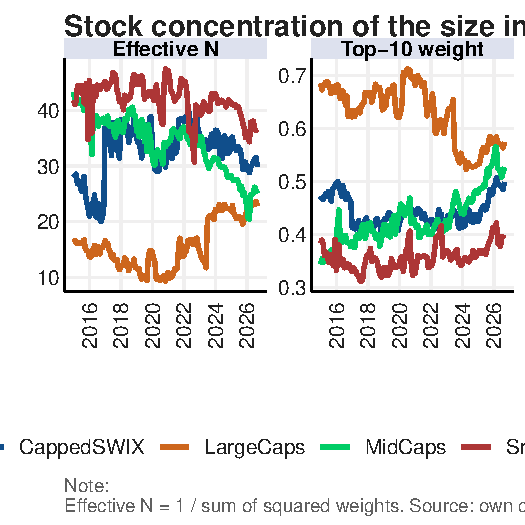
\includegraphics[keepaspectratio,alt={Stock concentration: top-10 weight and effective number of stocks }]{Question2_files/figure-latex/Figure2-1.pdf}}
\caption{Stock concentration: top-10 weight and effective number of
stocks \label{Figure2}}
\end{figure}

\begin{verbatim}
tab_print(Conc_Table %>% rename(Index = Fund, `Stocks (N)` = N, `Top-10 weight` = Top10,
                                `Effective N` = Eff_N),
          caption = "Concentration by period (averages)", label = "tab:conc", digits = 2)
\end{verbatim}

\begin{table}[!htbp]
\centering
\caption{Concentration by period (averages)} 
\label{tab:conc}
\begingroup\footnotesize
\begin{tabular}{llrrr}
  \hline
Index & Period & Stocks (N) & Top-10 weight & Effective N \\ 
  \hline
CappedSWIX & 1. 2015-2019 & 161.18 & 0.44 & 31.11 \\ 
  CappedSWIX & 2. 2020-2023 & 137.58 & 0.43 & 34.34 \\ 
  CappedSWIX & 3. 2024-2026 & 121.75 & 0.46 & 32.29 \\ 
  LargeCaps & 1. 2015-2019 & 41.30 & 0.66 & 13.70 \\ 
  LargeCaps & 2. 2020-2023 & 39.12 & 0.64 & 14.13 \\ 
  LargeCaps & 3. 2024-2026 & 40.69 & 0.55 & 21.97 \\ 
  MidCaps & 1. 2015-2019 & 57.05 & 0.39 & 38.10 \\ 
  MidCaps & 2. 2020-2023 & 52.23 & 0.43 & 33.72 \\ 
  MidCaps & 3. 2024-2026 & 41.91 & 0.50 & 26.87 \\ 
  SmallCaps & 1. 2015-2019 & 60.85 & 0.35 & 43.52 \\ 
  SmallCaps & 2. 2020-2023 & 58.67 & 0.36 & 41.62 \\ 
  SmallCaps & 3. 2024-2026 & 53.72 & 0.38 & 39.36 \\ 
   \hline
\end{tabular}
\endgroup
\end{table}

\subsection{Active share relative to the Capped
SWIX}\label{active-share-relative-to-the-capped-swix}

Large caps are increasingly close to the benchmark (Figure
\ref{Figure3}, Table \ref{tab:as}). Their active share halved, from 29\%
in 2015--19 to 15\% in 2024--26. A large-cap tilt therefore adds little
that is different from J433.

Mid and small caps are genuinely different portfolios, with active
shares of about 75\% and 93\%. Small caps hold stocks that make up only
about 7\% of the Capped SWIX, which makes them a true diversifier
relative to the benchmark.

One data feature is worth noting: in most months, about 12 stocks sit in
both the large- and mid-cap indexes at the same time, with a small
large-cap weight. This appears to reflect stocks migrating between size
bands; the weights are used as given.

\begin{verbatim}
fmxdat::finplot(g_as, x.date.dist = "1 year", x.date.type = "%Y",
                x.vert = TRUE, y.pct = TRUE, y.pct_acc = 1)
\end{verbatim}

\begin{figure}
\centering
\pandocbounded{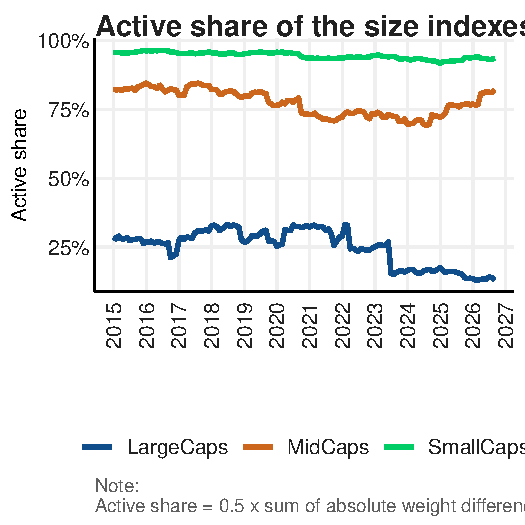
\includegraphics[keepaspectratio,alt={Active share of the size indexes relative to the Capped SWIX }]{Question2_files/figure-latex/Figure3-1.pdf}}
\caption{Active share of the size indexes relative to the Capped SWIX
\label{Figure3}}
\end{figure}

\begin{verbatim}
tab_print(AS_Table %>% rename(Index = Fund, `Active share` = Active_Share,
                              `Share of J433 weight held` = BM_Coverage),
          caption = "Active share relative to the Capped SWIX", label = "tab:as")
\end{verbatim}

\begin{table}[!htbp]
\centering
\caption{Active share relative to the Capped SWIX} 
\label{tab:as}
\begingroup\footnotesize
\begin{tabular}{llrr}
  \hline
Index & Period & Active share & Share of J433 weight held \\ 
  \hline
LargeCaps & 1. 2015-2019 & 0.287 & 0.778 \\ 
  LargeCaps & 2. 2020-2023 & 0.268 & 0.811 \\ 
  LargeCaps & 3. 2024-2026 & 0.152 & 0.848 \\ 
  MidCaps & 1. 2015-2019 & 0.818 & 0.182 \\ 
  MidCaps & 2. 2020-2023 & 0.735 & 0.265 \\ 
  MidCaps & 3. 2024-2026 & 0.752 & 0.248 \\ 
  SmallCaps & 1. 2015-2019 & 0.957 & 0.043 \\ 
  SmallCaps & 2. 2020-2023 & 0.942 & 0.058 \\ 
  SmallCaps & 3. 2024-2026 & 0.931 & 0.069 \\ 
   \hline
\end{tabular}
\endgroup
\end{table}

\subsection{Risk and return}\label{risk-and-return}

Table \ref{tab:stats} compares the indexes over the last ten years using
monthly returns.

\begin{itemize}
\tightlist
\item
  \textbf{Large caps} delivered the best balance of return and risk:
  11.6\% a year, a 22.6\% maximum drawdown and a beta of about one.
\item
  \textbf{Small caps} matched that return (11.4\%) with a beta of only
  0.73, but suffered the deepest drawdown (41.5\%).
\item
  \textbf{Mid caps} lagged, at 6.9\% a year.
\end{itemize}

\begin{verbatim}
tab_print(Tab_stats %>% filter(Period == "Last 10 Years") %>% select(-Period) %>%
            select(Info, LargeCaps, MidCaps, SmallCaps, CappedSWIX),
          caption = "Risk and return statistics, last 10 years (monthly returns, benchmark J433)",
          label = "tab:stats")
\end{verbatim}

\begin{table}[!htbp]
\centering
\caption{Risk and return statistics, last 10 years (monthly returns, benchmark J433)} 
\label{tab:stats}
\begingroup\footnotesize
\begin{tabular}{lrrrr}
  \hline
Info & LargeCaps & MidCaps & SmallCaps & CappedSWIX \\ 
  \hline
Cum Returns & 2.010 & 0.951 & 1.953 & 1.372 \\ 
  Returns (Ann.) & 0.116 & 0.069 & 0.114 & 0.090 \\ 
  Returns Excess (Ann.) & 0.024 & -0.019 & 0.022 & 0.000 \\ 
  SD (Ann.) & 0.154 & 0.153 & 0.144 & 0.145 \\ 
  Return / Risk & 0.795 & 0.516 & 0.827 & 0.672 \\ 
  Max Drawdown & 0.226 & 0.324 & 0.415 & 0.312 \\ 
  Pain Index & 0.037 & 0.060 & 0.064 & 0.049 \\ 
  Tracking Error & 0.049 & 0.077 & 0.105 & 0.000 \\ 
  Beta & 1.009 & 0.918 & 0.733 & 1.000 \\ 
  Up Capture & 1.276 & 0.800 & 0.492 & 1.000 \\ 
  Down Capture & 0.996 & 0.998 & 0.648 & 1.000 \\ 
  Modified CVaR (95\%, monthly) & -0.082 & -0.134 & -0.110 & -0.102 \\ 
   \hline
\end{tabular}
\endgroup
\end{table}

Rolling three-year returns (Figure \ref{Figure4}) show how consistent
these outcomes were.

\begin{itemize}
\tightlist
\item
  \textbf{Large caps beat the Capped SWIX in 96\% of three-year
  windows}, by about 2.5\% a year on average.
\item
  \textbf{Small caps won 64\% of the time but swung widely}, from
  \(-16\%\) a year in 2019--20 to about 37\% in 2022--23.
\item
  \textbf{Mid caps beat the benchmark in only 26\% of windows.}
\end{itemize}

\begin{verbatim}
fmxdat::finplot(g_rollret, x.date.dist = "1 year", x.date.type = "%Y",
                x.vert = TRUE, y.pct = TRUE, y.pct_acc = 1)
\end{verbatim}

\begin{figure}
\centering
\pandocbounded{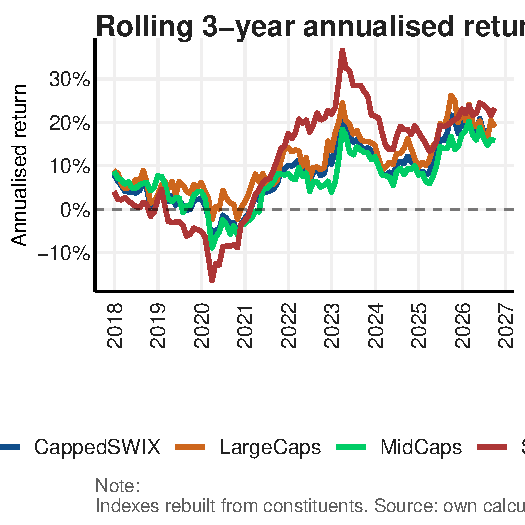
\includegraphics[keepaspectratio,alt={Rolling three-year annualised returns }]{Question2_files/figure-latex/Figure4-1.pdf}}
\caption{Rolling three-year annualised returns \label{Figure4}}
\end{figure}

\subsection{\texorpdfstring{Realised volatility
\label{Vol}}{Realised volatility }}\label{realised-volatility}

At index level, all three size indexes became much more volatile in 2020
(about 29--32\%), then settled (Figure \ref{Figure5}). Small caps were
consistently the calmest on daily data: about 12\% since 2024, against
17\% for large and mid caps.

\begin{verbatim}
fmxdat::finplot(g_rollsd, x.date.dist = "1 year", x.date.type = "%Y",
                x.vert = TRUE, y.pct = TRUE, y.pct_acc = 1)
\end{verbatim}

\begin{figure}
\centering
\pandocbounded{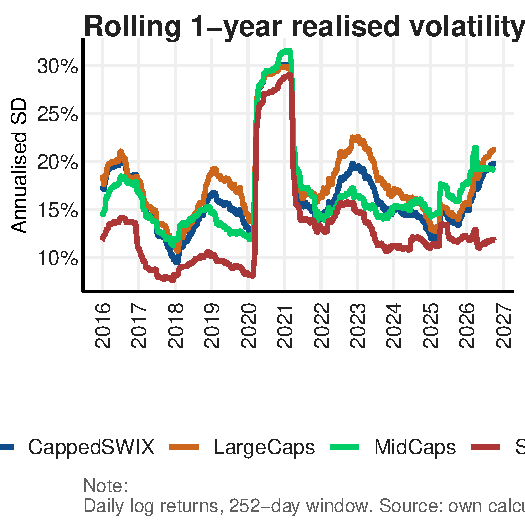
\includegraphics[keepaspectratio,alt={Rolling one-year realised volatility }]{Question2_files/figure-latex/Figure5-1.pdf}}
\caption{Rolling one-year realised volatility \label{Figure5}}
\end{figure}

The constituent view reverses this picture (Figure \ref{Figure6}, Table
\ref{tab:const}).

\begin{itemize}
\tightlist
\item
  \textbf{Individual small-cap stocks are the most volatile} (median of
  about 36\% in 2015--19, against 28\% for large caps).
\item
  \textbf{Yet the small-cap index is the calmest}, because its stocks
  move largely independently. Its diversification ratio is 0.28--0.41,
  against about 0.5 for large and mid caps.
\item
  \textbf{In 2020 the ratio rose sharply}: stocks moved together and
  diversification disappeared when it was needed most.
\end{itemize}

\begin{verbatim}
fmxdat::finplot(g_constrv, y.pct = TRUE, y.pct_acc = 1)
\end{verbatim}

\begin{figure}
\centering
\pandocbounded{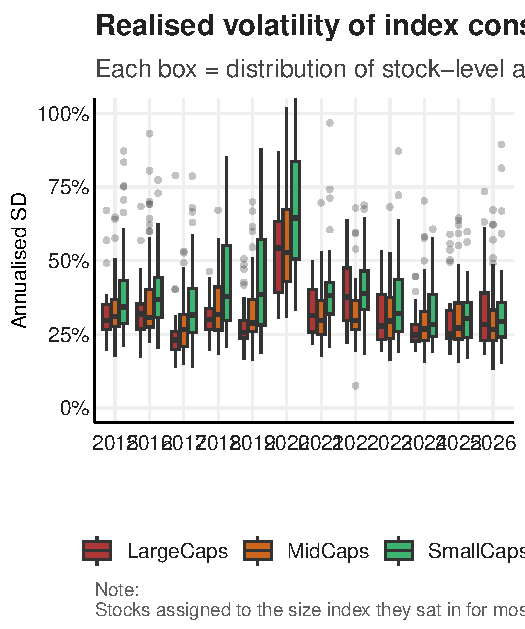
\includegraphics[keepaspectratio,alt={Distribution of constituent realised volatility by year }]{Question2_files/figure-latex/Figure6-1.pdf}}
\caption{Distribution of constituent realised volatility by year
\label{Figure6}}
\end{figure}

\begin{verbatim}
tab_print(Const_Period %>% rename(Index = Fund, `Median stock vol` = Median_Stock_RV,
                                  `Wtd. avg. stock vol` = WAvg_Stock_RV,
                                  `IQR stock vol` = IQR_Stock_RV, `Index vol` = Index_RV,
                                  `Diversification ratio` = Div_Ratio),
          caption = "Constituent versus index realised volatility", label = "tab:const",
          size = "\\scriptsize")
\end{verbatim}

\begin{table}[!htbp]
\centering
\caption{Constituent versus index realised volatility} 
\label{tab:const}
\begingroup\scriptsize
\begin{tabular}{llrrrrr}
  \hline
Index & Period & Median stock vol & Wtd. avg. stock vol & IQR stock vol & Index vol & Diversification ratio \\ 
  \hline
LargeCaps & 1. 2015-2019 & 0.280 & 0.298 & 0.072 & 0.162 & 0.538 \\ 
  LargeCaps & 2. 2020 & 0.542 & 0.486 & 0.241 & 0.298 & 0.613 \\ 
  LargeCaps & 3. 2021-2023 & 0.323 & 0.364 & 0.158 & 0.186 & 0.509 \\ 
  LargeCaps & 4. 2024-2026 & 0.260 & 0.330 & 0.104 & 0.171 & 0.511 \\ 
  MidCaps & 1. 2015-2019 & 0.298 & 0.331 & 0.117 & 0.140 & 0.421 \\ 
  MidCaps & 2. 2020 & 0.528 & 0.521 & 0.243 & 0.315 & 0.604 \\ 
  MidCaps & 3. 2021-2023 & 0.297 & 0.301 & 0.118 & 0.153 & 0.509 \\ 
  MidCaps & 4. 2024-2026 & 0.268 & 0.314 & 0.108 & 0.170 & 0.540 \\ 
  SmallCaps & 1. 2015-2019 & 0.357 & 0.355 & 0.194 & 0.099 & 0.278 \\ 
  SmallCaps & 2. 2020 & 0.645 & 0.613 & 0.331 & 0.288 & 0.470 \\ 
  SmallCaps & 3. 2021-2023 & 0.364 & 0.356 & 0.139 & 0.130 & 0.365 \\ 
  SmallCaps & 4. 2024-2026 & 0.293 & 0.288 & 0.125 & 0.118 & 0.408 \\ 
   \hline
\end{tabular}
\endgroup
\end{table}

Part of the small caps' calm is, however, an illusion (Table
\ref{tab:stale}).

\begin{itemize}
\tightlist
\item
  Small-cap stocks do not trade on about 11\% of days.
\item
  Small-cap daily index returns are positively autocorrelated.
\item
  Volatility measured on monthly returns is higher than on daily returns
  (ratio 1.06); for large caps the ratio is 0.80.
\end{itemize}

These are the signatures of stale prices. Daily small-cap volatility
understates true risk, which is consistent with the fat tails in Table
\ref{tab:desc} and the 41.5\% drawdown.

\begin{verbatim}
tab_print(Stale_Table %>% rename(Index = Tickers, `AC(1) daily` = AC1_daily,
                                 `SD from daily` = SD_from_daily,
                                 `SD from monthly` = SD_from_monthly,
                                 `Monthly / daily` = Ratio,
                                 `Zero-return days` = Zero_Return_Days),
          caption = "Stale-price diagnostics", label = "tab:stale")
\end{verbatim}

\begin{table}[!htbp]
\centering
\caption{Stale-price diagnostics} 
\label{tab:stale}
\begingroup\footnotesize
\begin{tabular}{lrrrrr}
  \hline
Index & AC(1) daily & SD from daily & SD from monthly & Monthly / daily & Zero-return days \\ 
  \hline
CappedSWIX & -0.003 & 0.173 & 0.141 & 0.810 &  \\ 
  LargeCaps & -0.018 & 0.186 & 0.150 & 0.804 & 0.016 \\ 
  MidCaps & 0.039 & 0.171 & 0.153 & 0.894 & 0.035 \\ 
  SmallCaps & 0.049 & 0.137 & 0.145 & 1.058 & 0.109 \\ 
   \hline
\end{tabular}
\endgroup
\end{table}

The GJR-GARCH estimates (Table \ref{tab:garch}, Figure \ref{Figure7})
add a further difference.

\begin{itemize}
\tightlist
\item
  \textbf{Large-cap volatility reacts almost only to bad news}
  (\(\alpha \approx 0\), \(\gamma = 0.15\)), like the Capped SWIX.
\item
  \textbf{Small and mid caps respond more symmetrically} (higher
  \(\alpha\), lower \(\gamma\)). Their volatility is driven more by
  stock-specific news than by market sell-offs.
\item
  \textbf{Shocks fade quickly} in all indexes, with half-lives of 12--18
  trading days.
\item
  \textbf{The models are adequate}: none of the Ljung--Box tests on
  squared standardised residuals rejects (\(p\) = 0.35 to 0.99).
\end{itemize}

\begin{verbatim}
fmxdat::finplot(g_sigma, x.date.dist = "1 year", x.date.type = "%Y",
                x.vert = TRUE, y.pct = TRUE, y.pct_acc = 1)
\end{verbatim}

\begin{figure}
\centering
\pandocbounded{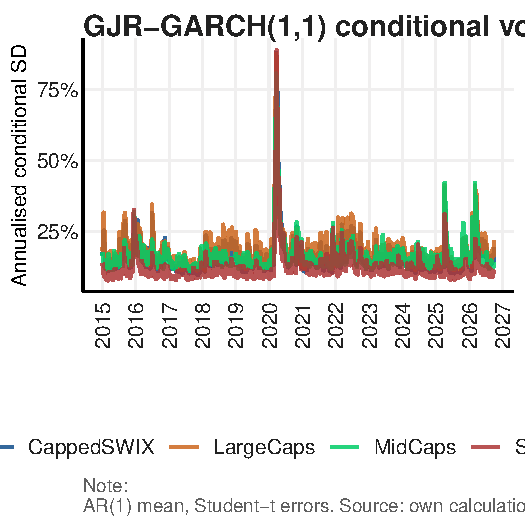
\includegraphics[keepaspectratio,alt={GJR-GARCH(1,1) conditional volatility }]{Question2_files/figure-latex/Figure7-1.pdf}}
\caption{GJR-GARCH(1,1) conditional volatility \label{Figure7}}
\end{figure}

\subsection{Stratification: calm versus stressed
months}\label{stratification-calm-versus-stressed-months}

Every size index becomes much more volatile in stressed months (Table
\ref{tab:stratsd}), so size offers no shelter from volatility. Small
caps react most to global fear (VIX), and mid caps least to local
stress. Global policy uncertainty barely changes volatility.

\begin{verbatim}
tab_print(SD_Results %>% select(Stratifier, Period, Tickers, Ratio) %>%
            pivot_wider(names_from = Tickers, values_from = Ratio) %>%
            select(Stratifier, Period, LargeCaps, MidCaps, SmallCaps, CappedSWIX) %>%
            arrange(Stratifier, Period),
          caption = "Volatility in extreme months relative to the full sample (ratio)",
          label = "tab:stratsd", digits = 2, size = "\\scriptsize")
\end{verbatim}

\begin{table}[!htbp]
\centering
\caption{Volatility in extreme months relative to the full sample (ratio)} 
\label{tab:stratsd}
\begingroup\scriptsize
\begin{tabular}{llrrrr}
  \hline
Stratifier & Period & LargeCaps & MidCaps & SmallCaps & CappedSWIX \\ 
  \hline
Global policy uncertainty & High & 1.05 & 1.15 & 1.11 & 1.09 \\ 
  Global policy uncertainty & Low & 0.98 & 0.97 & 0.92 & 1.02 \\ 
  J433 realised vol & High & 1.41 & 1.32 & 1.39 & 1.45 \\ 
  J433 realised vol & Low & 0.63 & 0.75 & 0.71 & 0.60 \\ 
  Oil realised vol & High & 1.25 & 1.17 & 1.19 & 1.28 \\ 
  Oil realised vol & Low & 0.80 & 0.85 & 0.89 & 0.78 \\ 
  Rand implied vol (SAVIUSD) & High & 1.16 & 1.17 & 1.16 & 1.20 \\ 
  Rand implied vol (SAVIUSD) & Low & 0.96 & 0.95 & 0.90 & 0.95 \\ 
  VIX & High & 1.31 & 1.29 & 1.38 & 1.33 \\ 
  VIX & Low & 0.76 & 0.84 & 0.74 & 0.75 \\ 
   \hline
\end{tabular}
\endgroup
\end{table}

Relative returns, however, depend on \textbf{local} stress only (Table
\ref{tab:strattt}, Figure \ref{Figure8}).

\begin{itemize}
\tightlist
\item
  \textbf{In calm months, large caps lead the market}, beating J433 by
  0.7\% a month in 68\% of months.
\item
  \textbf{In turbulent months, the leadership flips.} Mid and small caps
  beat J433 by about 0.8\% a month, while large caps lag in three out of
  four months.
\item
  \textbf{The differences are significant} for large caps (\(p = 0.01\))
  and mid caps (\(p = 0.02\)).
\item
  \textbf{Global stratifiers (VIX, oil, the rand, policy uncertainty)
  produce no significant size effect} (all \(p > 0.19\)). Global shocks
  hit all size segments similarly, so a size tilt is not a hedge against
  offshore uncertainty.
\end{itemize}

The small-cap result should be read with the stale-price caveat in mind:
lagged prices make falls look smaller. The mid-cap result does not
suffer from this.

\begin{verbatim}
tab_print(T_Tests %>%
            rename(Index = Tickers, `High minus Low (monthly)` = Diff_Hi_minus_Lo,
                   `p-value` = p_value),
          caption = "Monthly excess return over J433: High minus Low months (Welch t-test)",
          label = "tab:strattt", digits = 4, size = "\\scriptsize")
\end{verbatim}

\begin{table}[!htbp]
\centering
\caption{Monthly excess return over J433: High minus Low months (Welch t-test)} 
\label{tab:strattt}
\begingroup\scriptsize
\begin{tabular}{llrr}
  \hline
Stratifier & Index & High minus Low (monthly) & p-value \\ 
  \hline
Global policy uncertainty & LargeCaps & 0.0010 & 0.7382 \\ 
  Global policy uncertainty & MidCaps & -0.0089 & 0.1920 \\ 
  Global policy uncertainty & SmallCaps & -0.0020 & 0.8142 \\ 
  J433 realised vol & LargeCaps & -0.0092 & 0.0115 \\ 
  J433 realised vol & MidCaps & 0.0158 & 0.0217 \\ 
  J433 realised vol & SmallCaps & 0.0124 & 0.1121 \\ 
  Oil realised vol & LargeCaps & 0.0021 & 0.5606 \\ 
  Oil realised vol & MidCaps & 0.0060 & 0.3455 \\ 
  Oil realised vol & SmallCaps & 0.0067 & 0.4473 \\ 
  Rand implied vol (SAVIUSD) & LargeCaps & 0.0009 & 0.8033 \\ 
  Rand implied vol (SAVIUSD) & MidCaps & 0.0036 & 0.6459 \\ 
  Rand implied vol (SAVIUSD) & SmallCaps & -0.0063 & 0.4980 \\ 
  VIX & LargeCaps & 0.0006 & 0.8666 \\ 
  VIX & MidCaps & -0.0029 & 0.6950 \\ 
  VIX & SmallCaps & 0.0044 & 0.5959 \\ 
   \hline
\end{tabular}
\endgroup
\end{table}

\begin{verbatim}
fmxdat::finplot(g_strat, y.pct = TRUE, y.pct_acc = 0.1)
\end{verbatim}

\begin{figure}
\centering
\pandocbounded{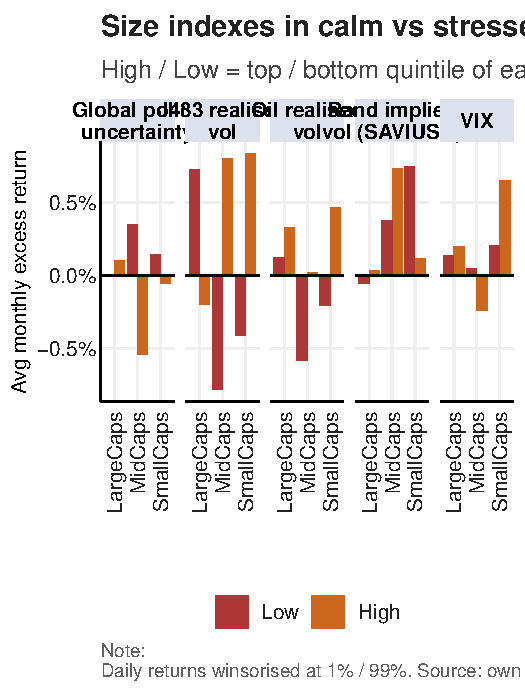
\includegraphics[keepaspectratio,alt={Average monthly excess return over J433 in calm and stressed months }]{Question2_files/figure-latex/Figure8-1.pdf}}
\caption{Average monthly excess return over J433 in calm and stressed
months \label{Figure8}}
\end{figure}

\section{\texorpdfstring{Model summary
\label{Summary}}{Model summary }}\label{model-summary}

Table \ref{tab:garch} summarises the volatility model, and Table
\ref{tab:summary} summarises the evidence from each technique.

\begin{verbatim}
tab_print(Garch_Table %>% rename(`gamma p-value` = gamma_p,
                                 `Half-life (days)` = Half_Life_days,
                                 `LB p (sq. resid.)` = LB_sq_p),
          caption = "GJR-GARCH(1,1) estimates: AR(1) mean, Student-t errors",
          label = "tab:garch")
\end{verbatim}

\begin{table}[!htbp]
\centering
\caption{GJR-GARCH(1,1) estimates: AR(1) mean, Student-t errors} 
\label{tab:garch}
\begingroup\footnotesize
\begin{tabular}{lrrrrrrrr}
  \hline
Index & alpha & beta & gamma & gamma p-value & shape & Persistence & Half-life (days) & LB p (sq. resid.) \\ 
  \hline
LargeCaps & 0.004 & 0.877 & 0.147 & 0.000 & 8.252 & 0.954 & 14.872 & 0.993 \\ 
  MidCaps & 0.035 & 0.869 & 0.080 & 0.000 & 7.963 & 0.944 & 12.050 & 0.529 \\ 
  SmallCaps & 0.062 & 0.850 & 0.073 & 0.025 & 7.138 & 0.948 & 13.107 & 0.352 \\ 
  CappedSWIX & 0.012 & 0.885 & 0.133 & 0.000 & 8.205 & 0.963 & 18.412 & 0.991 \\ 
   \hline
\end{tabular}
\endgroup
\end{table}

\begin{verbatim}
Summary_Tab <- tibble(
  Technique = c("Sector weights", "Concentration", "Active share",
                "Rolling returns", "Realised volatility", "Stale-price checks",
                "GJR-GARCH", "Stratification"),
  `Large caps` = c("Resources-heavy (35-40%)", "Most concentrated", "Low (15%): close to J433",
                   "Beat J433 in 96% of 3y windows", "Mid-range", "Clean",
                   "Strong bad-news effect", "Lead in calm months"),
  `Mid caps`   = c("Financials rising (28%)", "Rising concentration", "High (75%)",
                   "Beat J433 in 26% of windows", "Mid-range", "Minor",
                   "More symmetric", "Lead in stressed months"),
  `Small caps` = c("Property & Industrials", "Most diversified", "Very high (93%)",
                   "Volatile: -16% to +37% p.a.", "Lowest (index), highest (stocks)",
                   "Strong: vol understated", "Most symmetric", "Lead in stressed months*")
)
print(xtable::xtable(Summary_Tab, caption = "Summary of findings by technique",
                     label = "tab:summary",
                     align = c("l", "p{2.6cm}", "p{3.6cm}", "p{3.6cm}", "p{3.6cm}")),
      include.rownames = FALSE, comment = FALSE, table.placement = "!htbp",
      caption.placement = "top", size = "\\scriptsize")
\end{verbatim}

\begin{table}[!htbp]
\centering
\caption{Summary of findings by technique} 
\label{tab:summary}
\begingroup\scriptsize
\begin{tabular}{p{2.6cm}p{3.6cm}p{3.6cm}p{3.6cm}}
  \hline
Technique & Large caps & Mid caps & Small caps \\ 
  \hline
Sector weights & Resources-heavy (35-40\%) & Financials rising (28\%) & Property \& Industrials \\ 
  Concentration & Most concentrated & Rising concentration & Most diversified \\ 
  Active share & Low (15\%): close to J433 & High (75\%) & Very high (93\%) \\ 
  Rolling returns & Beat J433 in 96\% of 3y windows & Beat J433 in 26\% of windows & Volatile: -16\% to +37\% p.a. \\ 
  Realised volatility & Mid-range & Mid-range & Lowest (index), highest (stocks) \\ 
  Stale-price checks & Clean & Minor & Strong: vol understated \\ 
  GJR-GARCH & Strong bad-news effect & More symmetric & Most symmetric \\ 
  Stratification & Lead in calm months & Lead in stressed months & Lead in stressed months* \\ 
   \hline
\end{tabular}
\endgroup
\end{table}

\noindent \footnotesize\{* Subject to the stale-price caveat in Section
\ref{Vol}.\} \normalsize

The three size indexes offer distinct exposures:

\begin{itemize}
\tightlist
\item
  \textbf{Large caps} are a concentrated Resources and gold bet that has
  converged towards the Capped SWIX. They led the market over most of
  the sample and in calm months, but their volatility reacts sharply to
  bad news.
\item
  \textbf{Mid caps} are a Financials-tilted, increasingly concentrated
  portfolio far from the benchmark. They underperformed overall but held
  up best in locally stressed months.
\item
  \textbf{Small caps} are the most different from J433 and the most
  diversified internally. Their low measured volatility is partly a
  liquidity effect, and their tail risk is the largest.
\end{itemize}

For a manager benchmarked to the Capped SWIX, mid and small caps are the
source of genuine diversification, but against local stress, not
offshore uncertainty. Their measured risk should be judged on monthly
rather than daily data.

The main limitations are the missing sector labels for small caps, the
stocks that sit in both the large- and mid-cap indexes at the same time,
and the short sample of extreme months (28 per group) in the
stratification.

\newpage

\section*{References}\label{references}
\addcontentsline{toc}{section}{References}

\protect\phantomsection\label{refs}

\bibliography{Tex/ref}





\end{document}
